\documentclass[twocolumn]{article}
\usepackage[margin=1in]{geometry}
\usepackage{graphicx}
\graphicspath{ {C:/John/LaTeX/Scioly/Wright Stuff/Main/images/} }
\usepackage{grffile}
\usepackage{hyperref}

\title{Wright Stuff Event Guide}
\author{John Yang}
\date{March 25, 2019}

\begin{document}
\twocolumn[
\begin{@twocolumnfalse}
\maketitle
\begin{abstract}
Model airplanes are complex, multi-variable systems. In Wright Stuff, kits are allowed because the purpose of the event is not to design an aircraft, rather, the goal is for students to be able to learn how to test, assess, and adjust various parameters to achieve the highest degree of success. Here, we discuss the main principles of the event, and provide helpful resources so that you can get started quickly. 
\end{abstract}
\end{@twocolumnfalse}
]

\begin{figure}[h]
\caption{The 2019 Wright Stuff Freedom Flight Model Kit, by Dave Zeigler}
\centering
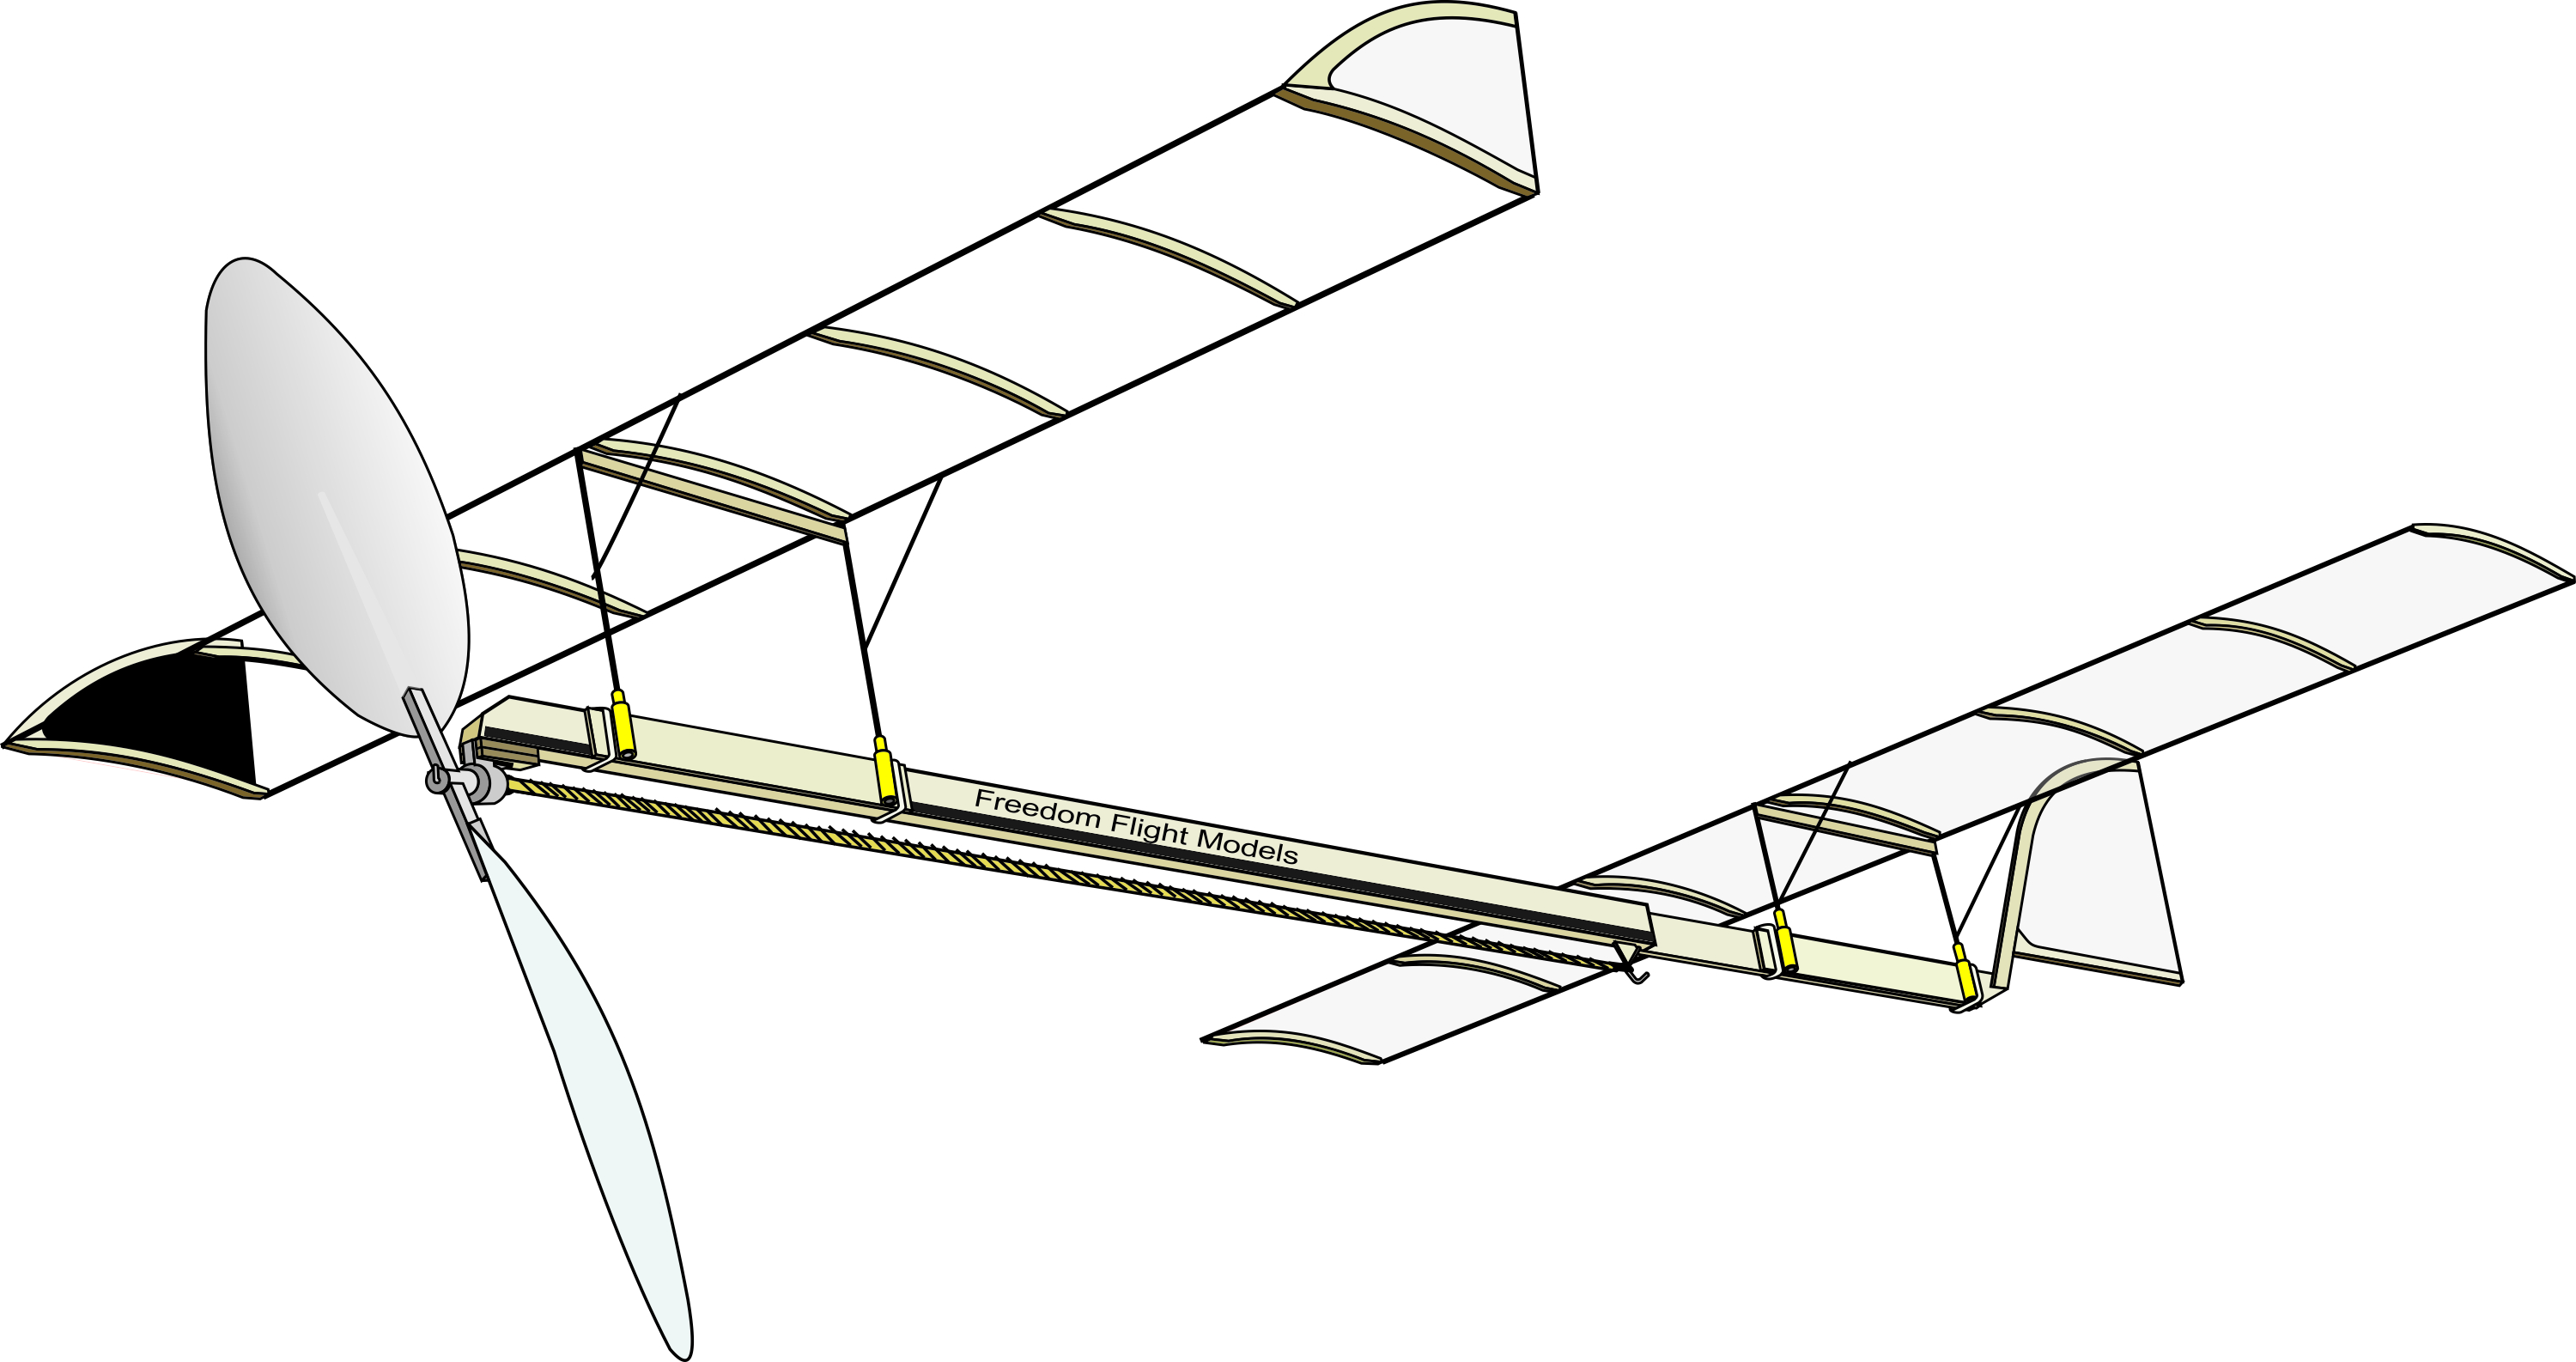
\includegraphics[scale=0.3]{FF plane}
\end{figure}

\section{A Brief Overview}
In case you haven't figured it out, Wright Stuff is an event where you build a model airplane, rubber powered. The required specs change every year, but the principle is mostly the same. The goal is always to keep the plane in the air for the longest amount of time, and this is done by building a quality aircraft and trimming it properly. 
\section{Terminology}
\textbf{Angle of Attack} - Angle of wing or stab relating to the air. \\
\textbf{Angle of Incidence} - Angle of wing or stab relating to the motorstick\\
\textbf{Bow} - When the motorstick bends vertically\\
\textbf{CA} - Cyanoacrylate glue (superglue)\\
\textbf{CF} - Carbon Fiber\\
\textbf{CG} - Center of Gravity\\
\textbf{Decalage} - Difference of angle between wing and stab. Positive when wing is higher than stab. \\
\textbf{Dive} - The plane flies nose-down and drops in altitude rapidly. \\
\textbf{Drag} - A force that points opposite to the velocity of an object moving through a fluid (in this case, air). The object pushes on air molecules, and the molecules push back, which is the drag. (Newton's 3rd Law)\\
\textbf{Motor} - Rubber\\
\textbf{Motorstick (``stick")} - Fuselage\\
\textbf{Prop Pitch} - Angle of the propeller. See trimming doc. \\
\textbf{Prop} - Propeller\\
\textbf{Radius} - Width of the plane's circle\\
\textbf{Stab} - Stabilizer\\
\textbf{Stall} - The nose lifts up so much that lift is lost because of turbulence over the wing. The nose lifts, then the plane loses speed, and then the nose drops again, allowing the wings to regain lift. \\
\textbf{Thrust} - Force that causes the airplane to accelerate forward. The propellers provide a force towards the rear of the airplanes, and the reaction force is the thrust. (Newton's 3rd Law again!)\\
\textbf{Torque} - Defined as the rotational analogue of force. For our purposes, torque is related to how much power the motor will provide, especially in the beginning of the flight. You can also think of it like this: Higher torque $=$ more elastic potential energy. (Yes, it's not the same but it is related). \\
\textbf{Trim Flight} - Non-official flight\\
\textbf{Trimming} - Adjusting factors in your plane to make it fly as long as possible. You MUST do this!! Countless practice flights are needed for success. See the trimming doc. \\
\section{Building}
Most teams use kits, and most of these teams use the Freedom Flight Models kit (Figure 1). These are usually the highest quality. However, it may be worthwhile to experiment with other kits such as the ``Senior Flyer" by Joshua Finn, and the ``Camp Robber" by John McGrath (Laser Cut Planes). Links are provided at the end of this document. The benefits to these kits are that they may be easier to build, and are much cheaper. Generally, kits are your best bet since they are relatively easy to build and have been tested by the designers. It's just up to you to be able to adjust it so that it flies well. However, if you have the necessary tools, and feel you are up to the challenge, feel free to build your own plane from scratch. If you understand Aerodynamics and know how to apply it, then you may be well served to build your own plane, with your own features. Another thing that experienced flyers do is modify kit components, or mix-and-match between kits. The purpose is to replace components that you don't like, and it could possibly help with reducing mass. 

When building, the most important thing is to follow the instructions, precisely. When the kit first arrives, before you do anything with it, read the instructions. Twice. Get a feel for the building process, and understand the purpose of each step. 

\section{Winding and Flying}
When making motors, use two o-rings or similar materials. Weigh out your rubber to the desired mass, with the o-rings on. Try to go .1 gram over before cutting. With the o-rings on, tie an overhand knot, plus two square knots, tightly. You may or may not also want to add some CA glue on the tip of the knot, if you are afraid that it will come loose. Cut off the two leftover pieces to about 1/32 inches. If there is a motor mass restriction, check to make sure you are slightly underweight before lubricating. 

When you are ready to fly, lubricate your motor using ArmorAll, or another lubricant. Place the motor into a snack-sized ziplock bag, and squirt a spray of lube into it. Rub it around and take out the motor. Do not leave the motor in the bag, as the lube can eat away at it. Feel the motor. If it feels to wet, you can shake it off to get rid of the excess. You don't want it to be dripping during flight, but you also don't want it to be too dry, as it might break. 

Use a geared winder, from Freedom Flight Models. The one with a blue tip has a 15:1 ratio and the one with a white tip has a 10:1 ratio. When winding, wind clockwise, and use the winder end as the side on the prop. Another option is to wind counterclockwise, and use that end as the rear. If you are winding the wrong way, you will be able to notice it when you fly. The plane will not turn correctly, and it may even turn clockwise. You want it to turn counterclockwise. See trimming doc. 

Torque meters may be helpful here, so that you can monitor the torque while winding. However, they are not necessary, as long as you count your winds and have a good feel for it. Stretch the motor to 4 times its natural length, and start winding. Again, remember to count your winds. At about 70\% of your winds, there will be so much torque that you might feel like the motor will break. From here, the goal is to keep the torque the same. Slowly start to walk in as you finish winding. If you are too slow, the torque will increase so much that it might break. Walk in too fast, and the rubber might knot up. If using a torque meter, keep the reading more or less constant. When you are finished, both partners should tightly grab their ends of the motor. Generally, the non-winding person will pick up the plane. The rear side goes on first, then the prop side. When the rubber is on, the person launching should hold the prop so that it doesn't spin. 

The launcher should walk to desired location, with one hand on the prop and the other at the CG location. When ready to fly, count off a 3...2...1... release. When counting, let go of the prop on 2, and on 1, accelerate the plane to walking speed, and let go. Do this gently. The plane does not need to fly very fast. The other partner should time. Aim for times above 2 minutes, but the longer the better. 
\section{Analysis of Flying Environment}
At competitions, do not fly first. Look at other teams, and notice air currents. It will be visible when there are air currents, as flights will be unsteady and rapidly increase and gain altitude. Details on how to adjust your plane to this are in the trimming doc. 

When choosing a launch location, keep in mind what your plane's radius usually looks like, and choose the path that has the least obstacles, INCLUDING AIR BLOWERS. You don't want to be unnecessarily affected by air currents, and you certainly don't want your flight to end early because you hit a wall or another obstacle. Check for celing obstacles, such as rafters and lights, and make a guess as to how tall the room is (unless they tell you - check the website beforehand). You will have to plan your flight accordingly, either by dewinding or using torque burners (See Torque Burners doc). 
\twocolumn[
\begin{@twocolumnfalse}
\section{Resources}
Freedom Flight Models - https://www.freedomflightmodels.com/\\
Laser Cut Planes - http://www.lasercutplanes.com/\\
Senior Flyer - http://jhaerospace.com/product/senior-flyer-2018-2019-div-c-contest-model/\\
Hip Pocket forum - http://www.hippocketaeronautics.com/hpa\_forum/index.php?board=33.0\\
2019 Scioly.org Forum - https://scioly.org/forums/viewforum.php?f=299\\
National Free Flight Society - https://freeflight.org/\\
INAV - https://indoornewsandviews.com\\
Wikipedia and Google are your best friends! (But you will have to dig a little deeper). 
\end{@twocolumnfalse}
]
\end{document}